\chapter{評価実験}\label{chap:evaluation}
全てのタスクにおいてネットワークはLSTMコントローラを採用し、ロジスティックシグモイド出力層を有する。
クロスエントロピーを損失関数として訓練し、最適化手法としてはAdamを用いた。
また、各入力系列の開始時にネットワークの隠れ状態はリセットされる。
各タスクにおけるネットワークのパラメータ、データのバッチサイズ、学習率を付録〜に示す。
実験1・2・4ではビットエラー数が1以下を記録した時点で、実験3では正答率が0.9以上を記録した時点でタスクを解決したとみなし実験を終了した。
\begin{comment}
複数のタスクでネットワークを評価する。実験の目的を以下に示す
\\・4.2節では順序整理モジュールの有効性をablation studyにより検証する
\\・4.3節では提案する非分散型メモリの長期依存関係の計算能力を分散型の既存手法と比較する
\\・4.4節では提案ネットワークにおける関係推論能力を評価する
\\・4.5節ではより複雑な関係推論を必要とするタスクにおける性能をベースラインの関係推論ネットワークと比較する
\end{comment}

\section{実験1 メモリ効率性の検証}
\subsection{実験概要}
NTMとSTMのメモリ操作における,メモリの容量を無駄なく使用する能力(以下メモリ効率性)を比較するためモデルのメモリサイズを揃えて性能を比較した。
評価にはNTM,STMの論文中でも実験で使用されたアルゴリズムタスクであるPriority Sortタスクを用いた。
NTMの論文中ではタスクの入力長が20であるのに対し行数128のメモリを用いて評価を行っている。
本実験ではメモリの容量に余裕のない状態での性能を評価したいため、付録〜に示すようにメモリの行数は入力長と同じ20とした。
比較するSTMのメモリサイズは提案ネットワークと同様に項目メモリ・関係メモリ共に20行とした。
ただしSTMは複数の関係メモリに並列して読み書きを行うことで豊かな関係情報を計算・保存することを長所にしており、
論文中で評価されたモデルでも関係メモリは項目メモリの8倍の大きさを持つ。
そこで関係メモリのサイズを8倍に設定したSTMにおいても実験を行い、性能を比較した。
また、実験1・2では各モデルにおいて2回ずつ独立した学習を行った。

\subsection{タスク:priority sort}
入力系列はランダムなバイナリベクトルに、[-1,1]の範囲から一様分布に従い決定した乱数を優先度として付加したものからなる。
ターゲットは入力系列をこの優先度に従ってソートした系列の一部とする。
NTM中の設定に従い入力系列の長さは20ベクトル,ターゲットは系列の中から優先度が高い順に16ベクトルとする。
評価指標にはビットエラー数を用いた。
これは正規化されたモデルの出力を0.5をしきい値として2値の予測系列に変換した上で、ターゲット系列と異なるビットの数をカウントしたものである。
図\ref{fig:priority}はpriority sortタスクの入力・ターゲットの構成を図示したものである。
\begin{figure}[t]
	\centering
	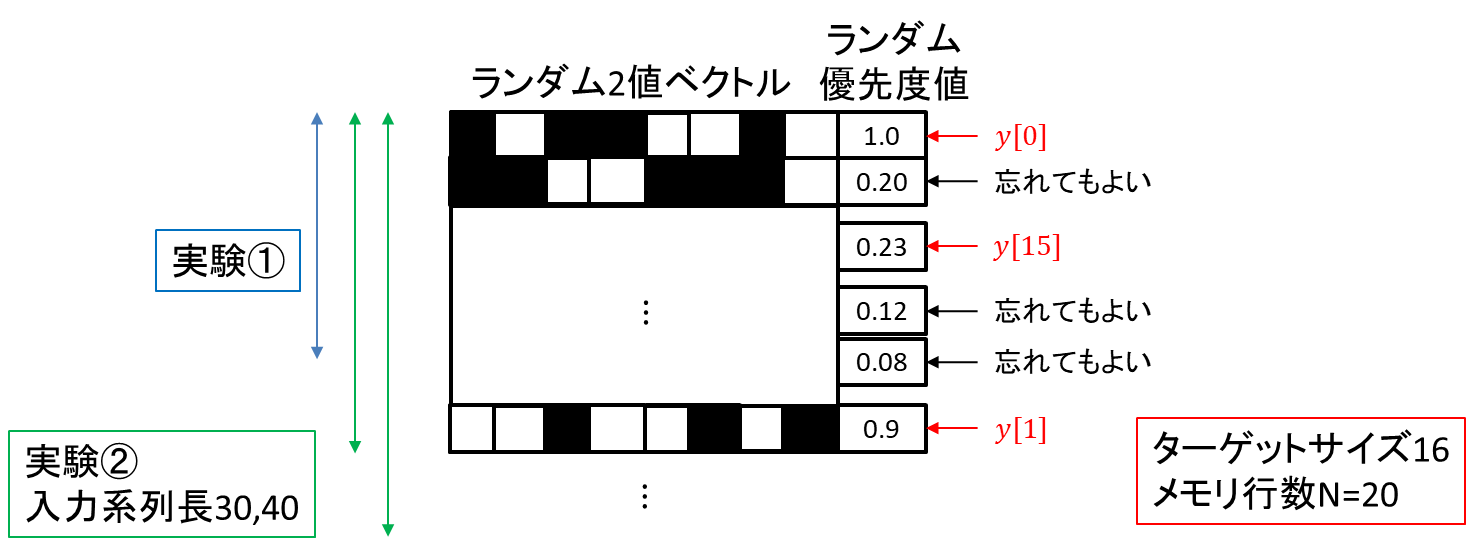
\includegraphics[width=\linewidth]{./figure/img_slide/priority.png}
	\caption{priority sort タスク}
	\label{fig:priority}
\end{figure}

\subsection{実験結果}
Priority SortタスクにおけるNTMおよび提案ネットワークの学習曲線を図\ref{fig:priority_rrnn_m20l20}に示す。
関係メモリが項目メモリと同サイズのSTMの学習曲線を図\ref{fig:priority_samx1_l20}に,
関係メモリサイズが8倍のときのものを図\ref{fig:priority_samx8_l20}に示す。
以後、同色の学習曲線は同一のパラメータ設定下での実験を表す。
\begin{figure}[t]
	\centering
	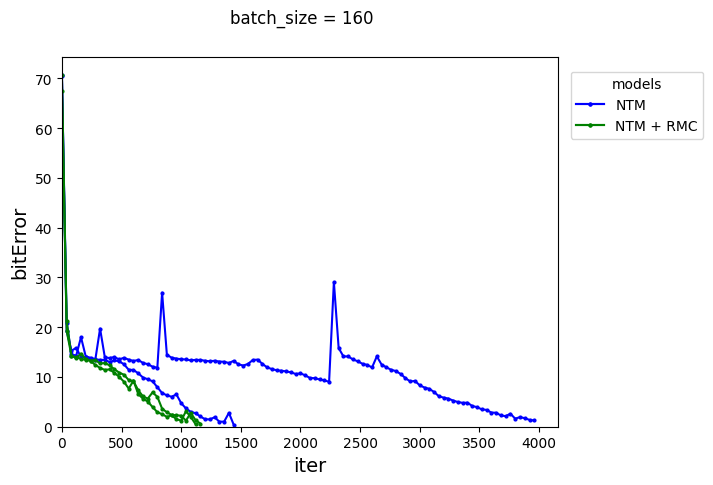
\includegraphics[width=\linewidth]{./figure/priority/rrnn_m20l20.png}
	\caption{NTMおよび提案ネットワークの学習曲線(入力長20)}
	\label{fig:priority_rrnn_m20l20}
\end{figure}
\begin{figure}[t]
	\centering
	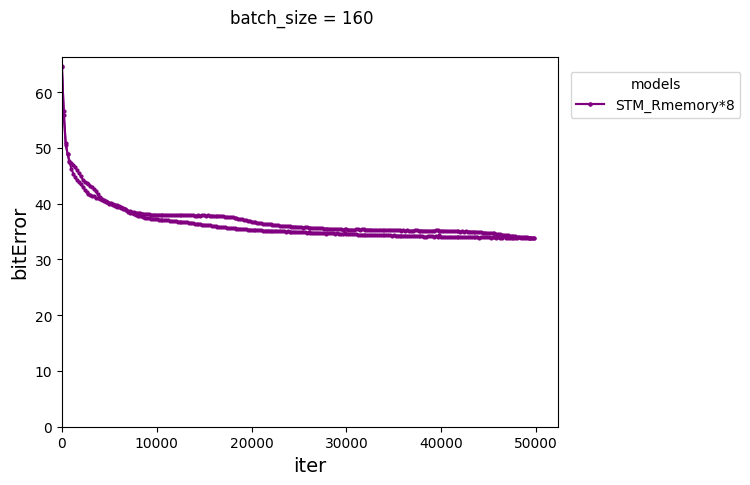
\includegraphics[width=\linewidth]{./figure/priority/samx1l20.png}
	\caption{STMの学習曲線(関係メモリ1倍・入力長20)}
	\label{fig:priority_samx1_l20}
\end{figure}
\begin{figure}[t]
	\centering
	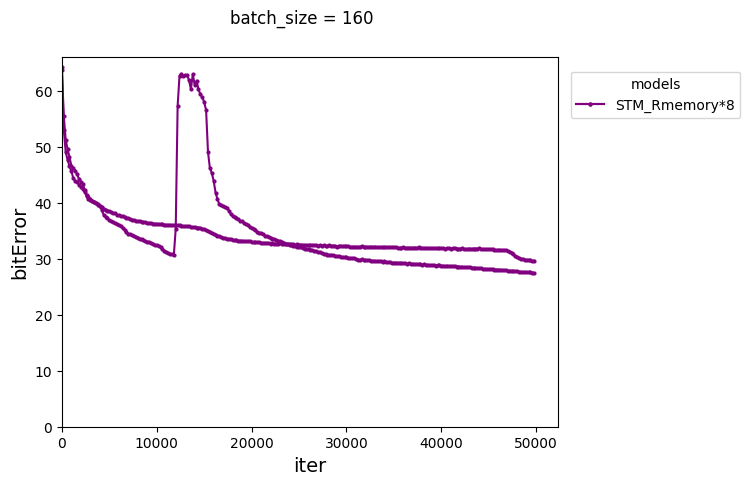
\includegraphics[width=\linewidth]{./figure/priority/samx8l20.png}
	\caption{STMの学習曲線(関係メモリ8倍・入力長20)}
	\label{fig:priority_samx8_l20}
\end{figure}

\subsection{考察}
既存研究よりも大幅にメモリサイズが削減された設定であったが、NTMおよび提案ネットワークはビットエラー数1を下回り、このタスクを解決することが出来た。
STMでは関係メモリのサイズに関わらず、NTM・提案ネットワークの10倍以上のイテレーションで学習した場合でもビットエラー数が30を下回ることは無かった。
これらの結果から、メモリ効率性においてNTMベースのメモリネットワークのSTMに対する優位性が示されたと考えられる。
またNTMは2回の学習のうち1回は学習に不安定性が見られ、収束までに約4000ほどのイテレーションを要した。
一方で提案ネットワークは安定して1200イテレーション未満で収束することに成功しており、これはNTMの最良の結果よりも早期の収束である。

\section{実験2 長期記憶・忘却能力の検証}
\subsection{実験概要}
Priority Sortタスクにおいて入力系列のサイズを増加させたときの精度の推移を観察する。
実験では入力長を30または40に設定した。
ターゲットサイズは16,メモリ行数は20から変更しないため、モデルは依然としてタスクの解決に必要な情報を全て保存する容量を有する。
しかし入力の初期に提示された情報を長期間記憶する能力や優先度の低い不要な項目を選択的に忘却しメモリを再利用する能力が要求される。

\subsection{実験結果}
入力長20,30,40でNTMを訓練したときの学習曲線を図\ref{fig:priority_ntm_m20_l20,30,40}に,
提案ネットワークを訓練したときのものを図\ref{fig:priority_rrnn_m20_l20,30,40}に示す。
同様に関係メモリが項目メモリと同サイズのSTMを訓練したときの学習曲線を図\ref{fig:priority_sam_x1_l20,30,40}に,
関係メモリサイズが8倍のときのものを図\ref{fig:priority_sam_x8_l20,30,40}に示す。
\begin{figure}[t]
	\centering
	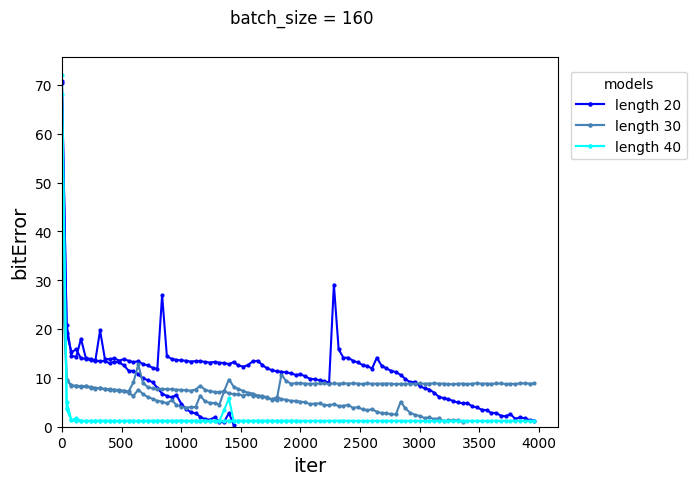
\includegraphics[width=\linewidth]{./figure/priority/ntm_m20_l20,30,40.png}
	\caption{NTMの学習曲線(入力長20,30,40)}
	\label{fig:priority_ntm_m20_l20,30,40}
\end{figure}
\begin{figure}[t]
	\centering
	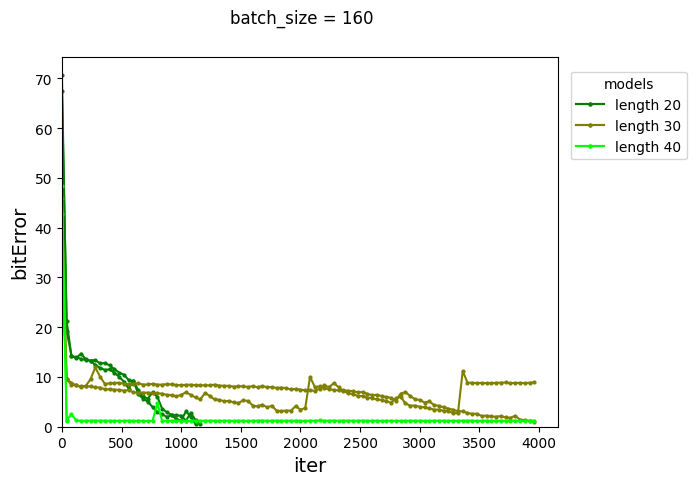
\includegraphics[width=\linewidth]{./figure/priority/rrnn_m20_l20,30,40.png}
	\caption{提案ネットワークの学習曲線(入力長20,30,40)}
	\label{fig:priority_rrnn_m20_l20,30,40}
\end{figure}
\begin{figure}[t]
	\centering
	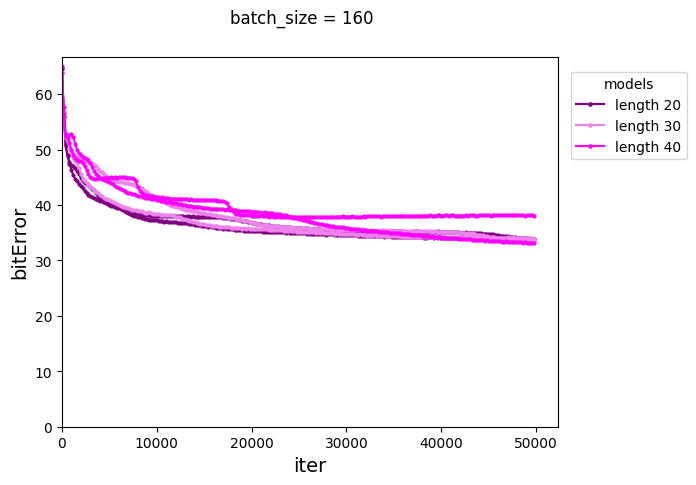
\includegraphics[width=\linewidth]{./figure/priority/sam_x1_l20,30,40.png}
	\caption{STMの学習曲線(関係メモリ1倍・入力長20,30,40)}
	\label{fig:priority_sam_x1_l20,30,40}
\end{figure}
\begin{figure}[t]
	\centering
	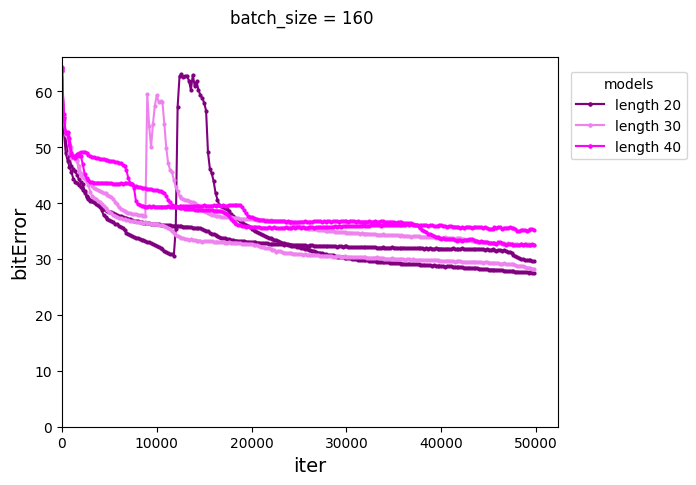
\includegraphics[width=\linewidth]{./figure/priority/sam_x8_l20,30,40.png}
	\caption{STMの学習曲線(関係メモリ8倍・入力長20,30,40)}
	\label{fig:priority_sam_x8_l20,30,40}
\end{figure}

\subsection{考察}
関係メモリが8倍のサイズを持つSTMでは、入力長の増加に伴いエラー率が増加することが読み取れる。
関係メモリが項目メモリと同サイズのSTMでは、イテレーション数が20000以下の範囲ではエラー率に増加が見られるが30000以上では収束し差がなくなる様子が確認できた。
NTMおよび提案ネットワークでは、入力長が30の場合は収束が大幅に遅くなりイテレーション数4000までに解決できない場合も確認された。
ただし、学習初期の500イテレーション以下でのエラー率は入力長20のケースよりも改善されており、最終的なエラー率もSTMの結果に勝っている。
入力長を40とした場合の学習では2回の学習共に非常に早期に収束し、モデルの解決能力は大幅に改善したと言える。

\section{実験3 関係推論能力の評価}
\subsection{実験概要}
この実験の目的は提案手法がNTMに関係推論能力を付与出来るかを評価することである。
実験で用いるNth-farthestタスクにおいて、
既存研究\cite{rrnn}\cite{sam}はRMCやSTMのような関係推論能力を持つモデルが90以上の精度を記録した一方で、NTMやDNCの精度は30を超えないことを示している。
提案ネットワークがNTMメモリ項目間の関係を計算できる場合、NTMよりも大きく改善された精度を示すことが期待される。

\subsection{タスク:Nth-farthest}
入力系列はランダムに生成されたバイナリベクトルからなる。
ベクトルの次元を$d$、系列長を$l$で表したとき、タスクの要求は入力系列中のあるベクトル$m$から$n$番目に遠いベクトルを見つける事である。
$m,n$は入力系列ごとにランダムに決定される。
1ステップあたりの入力はバイナリベクトル、ベクトルのID、$m$、$n$を連結したベクトルからなり、$ID,m,n∈\{1,2,…,l\}$はone-hotエンコーディングにより表現されるため、最終的な入力の次元は$d+3l$になる。
学習に時間を要する実験であったため、入力データの長さ・次元は既存研究\cite{rrnn}の半分の$d=8,l=4$とした。
それに伴い、メモリの大きさも既存研究の半分に設定した。
モデルは正答となるベクトルのIDを出力することを要求されるため、このタスクは分類問題である。評価指標には正答率を用いる。

このタスクは入力の読み書きやソートといったタスクよりも複雑な処理をネットワークに要求する。
ネットワークは$m$と全入力のペアの距離を計算しソートを行う必要がある。距離は入力間の関係情報の一形態である。
入力そのものをソートするタスクと異なり、関係情報のソートの為に関係メモリを活用する必要がある。

\subsection{実験結果}
Nth-farthestタスクによりRMCおよび提案ネットワークを訓練したときの学習曲線を図\ref{fig:nth_result}に示す。
\begin{figure}[t]
	\centering
	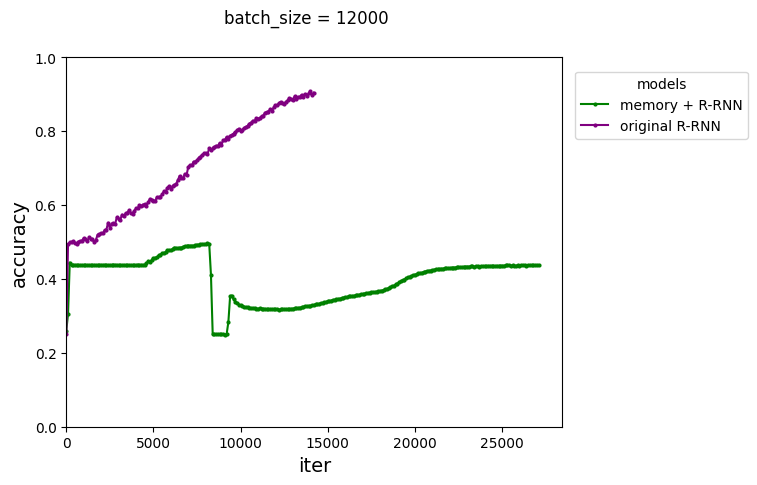
\includegraphics[width=\linewidth]{./figure/nth/orig_rrnn_id1.png}
	\caption{RMCおよび提案ネットワークの学習曲線}
	\label{fig:nth_result}
\end{figure}

\subsection{考察}\label{chap:nth-cons}
実験結果は提案ネットワークの精度は既存手法と異なり90\%に達することはなく、提案ネットワークに関係推論能力は確認されなかった。

原因の一つとして考えられるのは、関係メモリが受け取る情報が不足していたことである。
関係メモリが受け取る入力は項目メモリの保存内容のみであり、
NTMのヘッド内でメモリの更新や読み出しの判断に利用した情報を推論に用いることはない。
改善としてヘッド内で計算した値をメモリ操作を介さず直接関係メモリに渡す経路の追加が考えられる。
特に書き込み重みは、メモリの各行の内容を修飾するのに適した情報であると考えられる。

項目メモリ内の項目の順序に一貫性が無いことが、推論を妨げている可能性も考えられる。
\cite{working2mem}は非分散的に項目を格納する行列に関係推論をかける既存研究の例である。
この論文中のモデルは項目単位の忘却機構を持たず、入力系列に各時間ステップで埋め込みを適用したものを項目記憶として用いる
(論文中では短期記憶として記載されている)。
このため項目は提示された時刻に従って並ぶ一方で、
提案ネットワークでは項目の上書きが発生するため、項目の並び順に一貫性がなくなる可能性がある。
この問題を解決する方法としては、
時間順序に関する情報を別に保存し関係メモリに入力すること、あるいは
時間とは別の基準をもってメモリを一貫性を持った並びに変えることが有効であると考えられる。

また[NTM-implement]はNTMはハイパーパラメータが共通でも、収束までの時間がばらついたり収束に失敗したりする場合があることを指摘している。
提案ネットワークがこうしたNTMの不安定性を引き継ぎ、実験では偶然収束しなかった可能性も考えられる。
同一の設定で何度か追加で学習し、平均精度や収束した回数で評価する必要があると言える。

\section{実験4 関係推論能力改善の検証}
\subsection{実験概要}
\ref{chap:nth-cons}の考察を踏まえ、項目メモリへの書き込みに関する情報を用いて関係メモリの入力を改善し、項目メモリと関係メモリの連携を強化することを試みた。
実験では4種類の異なる方法で変更を加えたモデルの性能をNTMや提案ネットワークと比較し,評価した。
1つ目のモデルでは式\ref{eq:w_sum}で計算される,書き込み重みの総和$q_t$に基づき項目メモリをソートしたものを関係メモリへの入力とした。
このモデルではヘッドにおける計算の内容を直接提示することではなく、関係メモリの入力を一貫性を持った並びにすることを目的としている。
入力系列全体を通して頻繁に提示される項目ほどコンテンツベースの重みによる更新が発生し、$q_t$は大きな値になると考えられる。
そのため関係メモリ内のself-attention入力層の重みは常に同程度の出現頻度の項目を提示されることが期待される。
ヘッドが複数存在する場合、全ヘッドの$q_t$の総和に基づいてソートを行う。
実験4では各モデルにおいて3回ずつ独立した学習を行った。
\begin{equation}\label{eq:w_sum}
	q_t=\sum_t{w^w_t}
\end{equation}
2つ目から4つ目のモデルでは書き込みに関する情報を項目メモリに新たな列として追加し,関係メモリへの入力とした。
ヘッドが複数存在する場合、ヘッドごとに異なる列として追加される。
2つ目では書き込み重みの総和$q_t$を追加した。
3つ目では式\ref{eq:w_sum_thr},\ref{eq:thr}に示すように、書き込み重みの各要素にしきい値処理を適用した値の総和$c_t$を追加した。
書き込み重みの総和を用いる試みでは、一つの行に一つの項目が強く書き込まれた場合と、弱い強度で数回書き込まれた場合の区別を付けることが出来ない。
3つ目の試みは0.1以上の強度の書き込みを全て一度の書き込みとみなし、各行の書き込み回数を保存・利用することを意図したものである。
\begin{equation}\label{eq:w_sum_thr}
	c_t=\sum_tf(w^w_t)
\end{equation}
\begin{equation}\label{eq:thr}
	f(w^w_t)(i)=
	\begin{cases}
	1 & (w^w_t(i) \geq 0.1)\\
	0 & (w^w_t(i) < 0.1)
	\end{cases}
\end{equation}
4つ目では最後に書き込みが行われた時間ステップの情報を項目メモリに追加した。
入力項目が提示された順序の情報を保持し、推論に利用することを目的としている。
付与される時刻は0-1に正規化され、書き込みが行われたかどうかの判定は3つ目の試みと同じく0.1をしきい値とした。

%4.1.1節及び4.1.2節ではネットワークの基礎的な記憶と項目整理の能力を評価する。
%NTM\cite{ntm}の評価で用いられたシンプルなアルゴリズムタスクを説明する。

\subsection{タスク:associative recall}
NTM\cite{ntm}の評価で用いられたシンプルなアルゴリズムタスクの一つである。
一定の長さのランダムに生成されたバイナリベクトルからなる系列を1アイテムとし、
始めにネットワークにはランダムな数のアイテムが入力される。
入力アイテム系列が提示された後、クエリとして入力アイテムのうちの一つが改めて入力される。
この時ターゲットとして、入力アイテムの中でクエリアイテムの次に提示されたアイテムを取る。
各アイテムの間および入力とクエリの間にはデリミタを表すベクトルが挿入される。
NTM\cite{ntm}中の設定に従い、ベクトルの次元を6,1アイテムの長さを3とし、アイテムの数は一様分布を用いて2-6のいずれかに決定する。
評価指標にはPriority Sortと同様にビットエラー数を用いる。

%以上の設定から入力系列の長さはデリミタを含め7-23,デリミタを除いた保存が必要な必要なベクトルに限ると6-18となる。既存研究\cite{ntm}ではメモリ行数は128に設定されており,これは全ての入力を順に保存するのに十分な。同じメモリ行に本実験では行数を12に設定した。

タスクはクエリアイテムをメモリから検索する、入力ベクトルを忠実に復元するといったメモリネットワークの基礎的な能力を要求する。
加えて、入力アイテムの順序の情報を保存する能力も要求する。

\subsection{実験結果}
Associative RecallタスクによりNTMおよび提案ネットワークを訓練した場合の学習曲線を図\ref{fig:ntm,rmc_m12id3}に示す。
\begin{figure}[t]
	\centering
	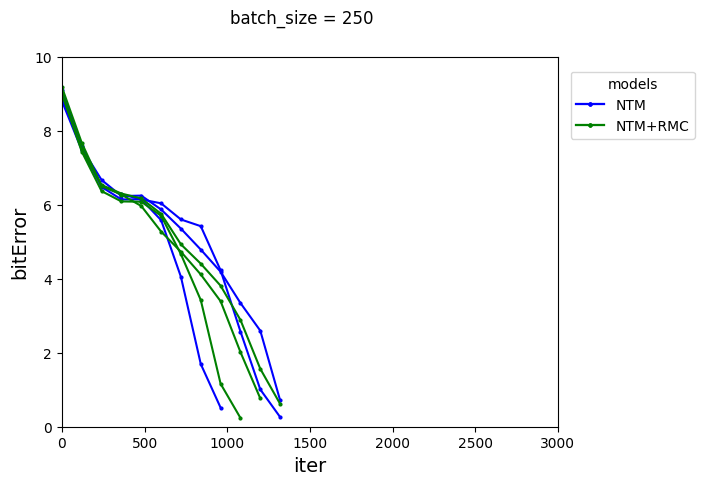
\includegraphics[width=\linewidth]{./figure/associative/ntm,rmc_m12id3.png}
	\caption{NTMおよび提案ネットワークの学習曲線}
	\label{fig:ntm,rmc_m12id3}
\end{figure}

書き込み重みの総和を付与した場合,および総和に従いソートを行った場合の学習曲線をNTMのものと共に図\ref{fig:ntm,sort,supple1}に示す。
各行の書き込み回数,最後に書き込んだ時刻を付与したモデルの学習曲線を図\ref{fig:ntm,supple2,3}に示す。
\begin{figure}[t]
	\centering
	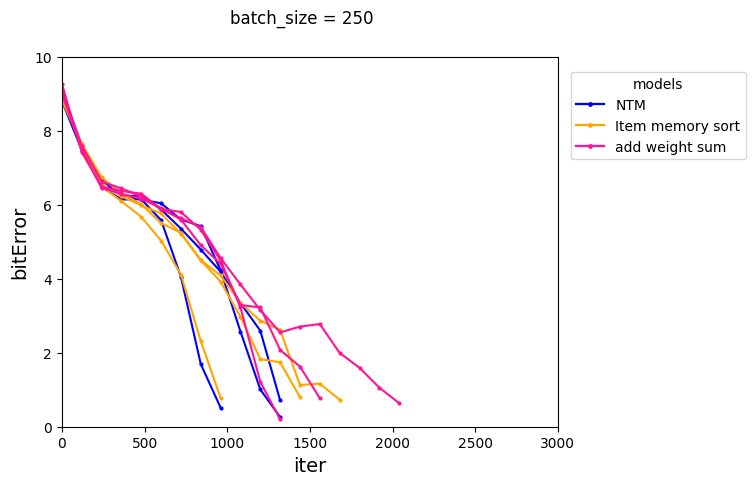
\includegraphics[width=\linewidth]{./figure/associative/ntm,sort,supple1_m12.png}
	\caption{書き込み重みの総和の付与,および総和に従ったソートを行ったときの学習曲線}
	\label{fig:ntm,sort,supple1}
\end{figure}
\begin{figure}[t]
	\centering
	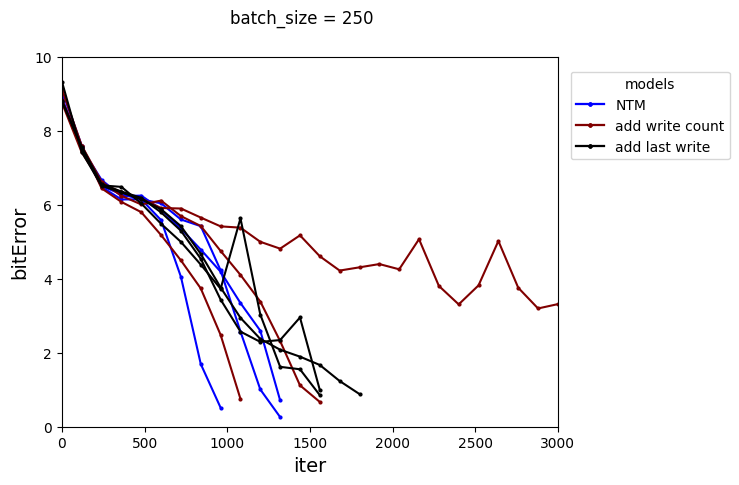
\includegraphics[width=\linewidth]{./figure/associative/ntm,supple2,3_m12.png}
	\caption{各行の書き込み回数,最後に書き込んだ時刻の付与を行ったときの学習曲線}
	\label{fig:ntm,supple2,3}
\end{figure}

\subsection{考察}
結果からこのタスクにおいては、NTMと提案ネットワークの間に顕著な違いは確認されなかった。
重みの総和に基づくソートでも、平均して学習曲線に大きな変化はなかった。
重みの総和あるいは最後に書き込んだ時刻を付与した場合は,平均してエラー率の収束は遅くなったことが読み取れる。
書き込み回数を付与した場合,3回中2回の学習ではNTMに大きくは劣らなかったが1回では収束が大幅に遅れ,モデルの安定性に悪影響を与えたと考えられる。

唯一NTM・提案ネットワークから性能にほぼ悪化が無かったソートを適用したモデルでは、関係メモリの入力の列数に変化はなかった。
性能が悪化した3つのモデルでは関係メモリのサイズに変化はない一方で、各行への書き込みに関する情報として項目メモリに新たな列を付加していた。
これらを比較すると、付加した情報が余分な情報として他の情報が保存されるスペースを圧迫してしまったことが性能悪化の一因と考えられる。
改善として付加される列数=ヘッド数の分関係メモリのサイズを増加させることが考えられる。

最後に書き込んだ時刻および書き込み回数に改善が見られなかった一因として、しきい値処理が逆伝播不可な操作であることも考えられる。
メモリ操作をスキップしてヘッドの情報を関係メモリに渡すことを目的とした操作だが、スキップした接続を通して書き込み重みの計算を最適化可能にする点に改善の余地がある。
しきい値の代わりに急峻なsigmoid関数のような微分可能関数を適用した場合との比較も今後行いたい。

%項目メモリのソートが変化がないのが以外だった。
%self-attentionの変換の重みは位置により機能が分化すると思っていたので。改善か悪化すると思っていた

\begin{comment}
	また,ああああああ


\begin{table}[H]
	\caption{あああといいいの予測誤差}
	\centering
	\scalebox{0.98}[0.98]{
		\begin{tabular}{c|c|c|c|c|c|c}
			\multicolumn{1}{c}{} & \multicolumn{2}{|c|}{2019} 
			& \multicolumn{2}{c|}{2018} & \multicolumn{2}{c}{2017}\\ \hline \hline
			モデル    & ああ & いい & ああ & いい & ああ & いい \\ \hline
			Naive    & \bf{1} & 1 & \bf{1} & 1 & \bf{1} & 1 \\
			TCN      & 1.0895 & 0.9032 & 1.4791 & \bf{0.9198} & 1.2888 & 0.8555 \\
			LSTM     & 1.0384 & 0.9295 & 1.4917 & 0.9725 & 1.1627 & 0.8541 \\
			提案手法  & 1.0977 & \bf{0.8698} & 1.3824 & 0.9439 & 1.2061 & \bf{0.8516} \\
		\end{tabular}
	}
	\label{table:result-1}
\end{table}

\end{comment}